\chapter{Background}
Ants are social insects that have evolved millions of years. Their strategies to find resources for their survival are fascinating. prior works describes several experiments on desert harvester ants at the field to observe how they forage\cite{flanagan2012quantifying}. Three different species of harvester ants are \textit{P. rugosus}, \textit{P. desertorum} and \textit{P. maricopa}.\par
Our goal was to figure out how these ants find resources from an environment and what is the effect of the distribution of seeds on which foraging behavior is used. Seeds in the fields are distributed in a  ring showning figure 2.1. The area of the food distribution is scaled with the colony size of ants. For example, \textit{Desertorum} was the smallest in colony size (77$\pm$296), so the  ring radius of food was 1.5 to 3 meters. \textit{Rugosus} has a colony size of 1712$\pm$174. So the radius of food distribution for \textit{Rugosus} was in 5-10 meters. The seeds are organized in a power law distribution around the nest.
\section{\label{section:Power Law}Power Law}
In power law distribution of food, seeds are distributed into multiple piles of different pile size. For example, 1024 seeds can be divided into four pile size categories with 256 seeds in each. One large pile of 256 seeds are placed all together in a random location in the ring. Next 256 seeds are divided into 4 equal sizes of 64 seeds and placed in the ring. Next 256 seeds are equally divided into 16 piles of 16 seeds and placed inside the ring. The remaining seeds are distributed uniformly around the nest.
\begin{figure}[h]
	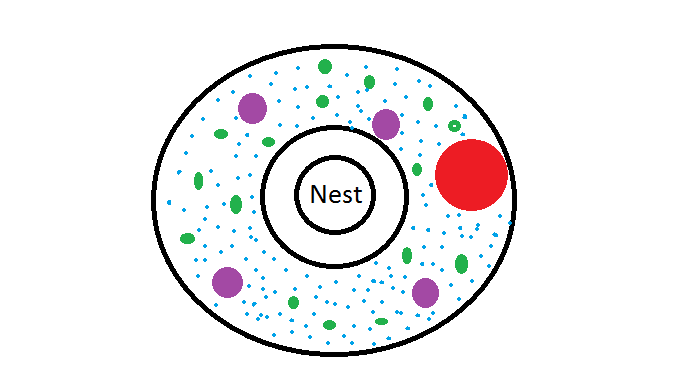
\includegraphics[width=\textwidth]{DonutShape.png}
	\caption{Distribution of Seeds in the field experiment for power law distribution with 1024 seeds. Red pile indicates one large pile of 256 seeds. 4 purple piles represent 4 large piles of 64 seeds, green color represents 16 piles of 16 seeds and blue seeds are 256 random seeds}
\end{figure}
\section{\label{section:CPFA}CPFA}
Central Place Foraging Algorithm(CPFA) is an agent-based model where agents are programmed to follow an ant inspired strategy to collect seeds. In CPFA, ants follow three methods to collect seeds\cite{hecker2015beyond}.
\begin{itemize}
	\item \textbf{Random Walk:} Ants starts walking randomly from the nest. If they find any food they bring it back to nest
	\item \textbf{Use of Internal Memory:} They remember the last position where the food was found and can return to that place for further search of food. This is method is called site fidelity.
	\item \textbf{Use of Pheromone or Communication:} They lay  pheromone trails from the food source to the nest so that other ants can follow that trail to collect food from that source.	
\end{itemize} 
Initially, a search location is selected for each of the ants. Then ants start traveling to the search site. After reaching the search site, they perform either uninformed random walk to a random location or informed random walk to a known location based on site fidelity or pheromone. If no resource is found, then they return to the nest.\par
If they find any resource they sense the local resource density. Based on the local resource density they decide whether to use site fidelity in future or to lay pheromone. After sensing the resource density, the return to the nest with the seed.\par
Whether the agents will use any of three strategies is governed by seven parameters. Table $2.1$ represents the seven parameters, that govern CPFA and their initialization values\cite{hecker2015beyond}.\par
\begin{table}[h]
	\begin{tabular}{ |p{0.6\textwidth}|p{0.33\textwidth}| } 
		\hline
		\textbf{Parameters} & \textbf{Initialization Functions} \\
		\hline 
		Probability of Switching to Searching & U(0,1)\\ 
		\hline
		Probability of Returning to Nest & U(0,1)\\ 
		\hline
		Uniform Search Variation & (0, 4 PI)\\
		\hline
		Rate of Informed Searched Decay & E(20,0)\\
		\hline
		Rate of Site Fidelity & E(20,0)\\
		\hline
		Rate of Laying Pheromone & E(20,0)\\
		\hline
		Rate of Pheromone Decay & E(20,0)\\
		\hline
	\end{tabular}
	\caption{Seven parameters and their initialization, that characterizes Central Place Foraging Algorithm}
\end{table}
For parameters in a uniform distribution, higher the value of the parameter the higher the probability of that event. For example, ``probability of switching to searching'' follows a uniform distribution. Higher values of this parameter, create a higher probability that the ant will switch to search from initial departure. \par
For the exponential distribution, the higher the value of the parameter, the lower the chance of using that feature. For example, if \textit{Rate of Laying Pheromone} is zero, then it means that there is a higher chance of laying the pheromone. On the other hand,  a value close to 20 means that chance of using the pheromone is very low.\par 
Ants determine the position of a search location by either using site fidelity, or pheromone or randomly. When they travel to a particular location, they look for resources. The \textit{probability of switching to searching} determines the chance of ants to switch to search for resources. When ants were not primed by site fidelity or pheromone information, they select a random direction to travel and search for resources in that direction. The higher the value of switching to the search, the faster they begin the search process.\par 
The \textit{probability of returning to nest} defines the chances of returning to nest for unsuccessful foraging trip. This parameter actually decides how long the ant will keep searching new places before returning to the nest. Higher the value of the parameter, mean that ants search shorter before returning to the nest..\par 
The \textit{rate of site fidelity} comes into play when the ants use site fidelity to go to an informed location where that ant remembers that the food already exists. The lower the value of this parameter, the higher the chances of following the site fidelity. \par 
The \textit{rate of laying pheromone} is the probability of laying pheromone while returning to nest from a food location. This depends on sensing of local resource density. When the ants collect seeds from a location, they sense the density of resources in nearby areas. Lower the value of \textit{probability of laying pheromone}, higher the chances of laying pheromone. \par 
The \textit{probability of pheromone decay} determines how fast the pheromone will evaporate. When the value of the parameter is high pheromone stays in the ground for a longer time. The pheromone evaporates faster for the lower value of the parameter.
\section{\label{section:Genetic Algorithm}Genetic Algorithm}
Genetic Algorithms are metaheuristic search algorithm inspired from natural selection and evolutionary genetics. As such they represent intelligent exploitation of a random search used to solve optimization problems. The basic techniques of GA’s are designed to simulate processes in natural systems necessary for evolution.\par
The evolution usually starts from a population of randomly generated individual strings that are analogous to the chromosome that we see in our DNA, and is an iterative process, with the population in each iteration called a generation. GAs simulate the survival of the fittest among individuals over the consecutive generation for solving a problem. Each individual represents a point in a search space and a possible solution. The individuals in the population are then made to go through a process of evolution. GA proceeds through the solution domain by evaluating the fitness function. 
The whole process of evolution is divided into three major section- selection, crossover \& mutation.

In our genetic algorithm, the strings that undergo mutation represents the seven parameters of CPFA. Mutation rate is fixed to one percent. \par 
The process is followed until a common termination condition is reached. This termination condition can be either a solution which fulfills minimum criteria. GA can also be terminated once it reaches a desired number of generation, or if it reaches the maximum fitness. Evaluation of fitness functions also takes lots of time. So sometimes the GA is bound to a strict time limit, in this case 50 generations.  The GA can also be terminated by any combination of the termination methods mentioned above.
GA Algorithm can be defined as \textit{algorithm 2.1}\\
\begin{algorithm}[H]
	\begin{algorithmic}[1]
	\State Initialize the population randomly
	\State Determine the fitness of the first generation
	 \While{Desired solution is obtaind}
	 		\State Select elite population with the best fitness
	 		\State Create a new population by crossover and mutation among the elite population
	 		\State Evaluate fitness of the population
		\EndWhile
		\caption{Genetic Algorithm at a glance.}
		\label{Genetic Algorithm at a glance.}
	\end{algorithmic}
\end{algorithm}
